% !TeX spellcheck = en_GB
\PassOptionsToPackage{implicit=true}{hyperref}
\documentclass[10pt, aspectratio=1610, compress, protectframetitle, handout]{beamer}
\usefonttheme{professionalfonts}
\setbeamertemplate{blocks}[rounded][shadow=true]
\usepackage[normalem]{ulem}
\usepackage[T1]{fontenc}
\usepackage{graphicx}
\usepackage{wrapfig}
\usepackage{float}
\usepackage{datetime}
\usepackage{textpos}
\usepackage{xcolor}
\usepackage{bm}
\usepackage[ruled,vlined]{algorithm2e}
\usepackage[autostyle]{csquotes}
\usepackage[export]{adjustbox}
\MakeOuterQuote{"}
\usepackage[]{enumitem}
\usepackage{appendixnumberbeamer}
\usepackage[british]{babel}
\usepackage{wrapfig}
\usetheme[titleformat=regular, sectionpage=progressbar, subsectionpage=none, numbering=fraction, progressbar=frametitle, block=fill]{metropolis}
\setmonofont{FiraMono-Regular.otf}

\graphicspath{{img/}}

\definecolor{MetroLinks}{RGB}{96, 76, 56}
\definecolor{MetroCite}{RGB}{35, 55, 59}
\definecolor{MetroUrl}{RGB}{20, 176, 61}

\hypersetup{
    colorlinks,
    linkcolor=MetroLinks,
    citecolor=MetroCite,
    urlcolor=MetroUrl,
}

% Change Colors/Width of Progress Bars
\makeatletter
\setlength{\metropolis@progressonsectionpage@linewidth}{3pt}
\makeatother


\title{\textsc{\texttt{C}ounter\texttt{A}dversarial \texttt{R}ecall of \texttt{S}ynthetic \texttt{O}bservations}}
\subtitle{A \textit{neuro-inspired} approach to foil gradient-based adversarial attacks}
\author{Emanuele \textsc{Ballarin}\inst{$\dagger$}}
\institute[]{
    \inst{$\dagger$} \scshape{\texttt{AICPS} $\in$ Dept. of Mathematics $\subseteq$ Univ. of Trieste} |
    \inst{$\ddagger$} \scshape{\texttt{AREA} Science Park}
}

\AtBeginSection[]
{
    \begin{frame}
        \frametitle{\textit{We are here}}
        \tableofcontents[currentsection]
    \end{frame}
}


\begin{document}
    % !TeX spellcheck = en_GB

\setbeamertemplate{title page}{
    \begin{minipage}[b][\paperheight]{\textwidth}
        \ifx\inserttitlegraphic\@empty\else\usebeamertemplate*{title graphic}\fi
        \vfill
        \ifx\inserttitle\@empty\else\usebeamertemplate*{title}\fi
        \ifx\insertsubtitle\@empty\else\usebeamertemplate*{subtitle}\fi
        \usebeamertemplate*{title separator}
        \vspace*{4px}
        \begin{minipage}[]{0.5\textwidth}
            \ifx\beamer@shortauthor\@empty\else\usebeamertemplate*{author}\fi
            \vspace*{1.8em}
        \end{minipage}
        \begin{minipage}[]{0.5\textwidth}
            \raggedleft
            {\small Supervised by: Prof. Luca \textsc{Bortolussi}{${}^\dagger$} \par}
            \vspace*{0.2em}
            {\small CoSupervised by: Dr. Alessio \textsc{Ansuini }{${}^\ddagger$}}
        \end{minipage}
        \vspace*{7px}
        \center\small Graduation session: M.Sc. in \textit{Data Science and Scientific Computing}
        \center\ifx\insertdate\@empty\else\usebeamertemplate*{date}\fi
        \vspace*{14px}
        \raggedright\ifx\insertinstitute\@empty\else\usebeamertemplate*{institute}\fi
        \vspace*{15px}
    \end{minipage}
}

\frame{\titlepage}

    % !TeX spellcheck = en_GB

\section{Minimal introduction to \textit{Deep Learning}}{
}

\section{The problem of \textit{adversarial robustness}}{
}

\section{\textit{(relatively}) Robust neural systems: \textit{brains}}{
}

\section{\texttt{CARSO}: an \textit{introspective artificial neural machine}}{
}

\section{Experimental evaluation}{
}

\section{Discussion}{
}

\section{Conclusion and future outlook}{
}
    % !TeX spellcheck = en_GB
\phantomsection
\begin{frame}{Thanks for your attention!}
    \centering
    \vspace*{15px}
    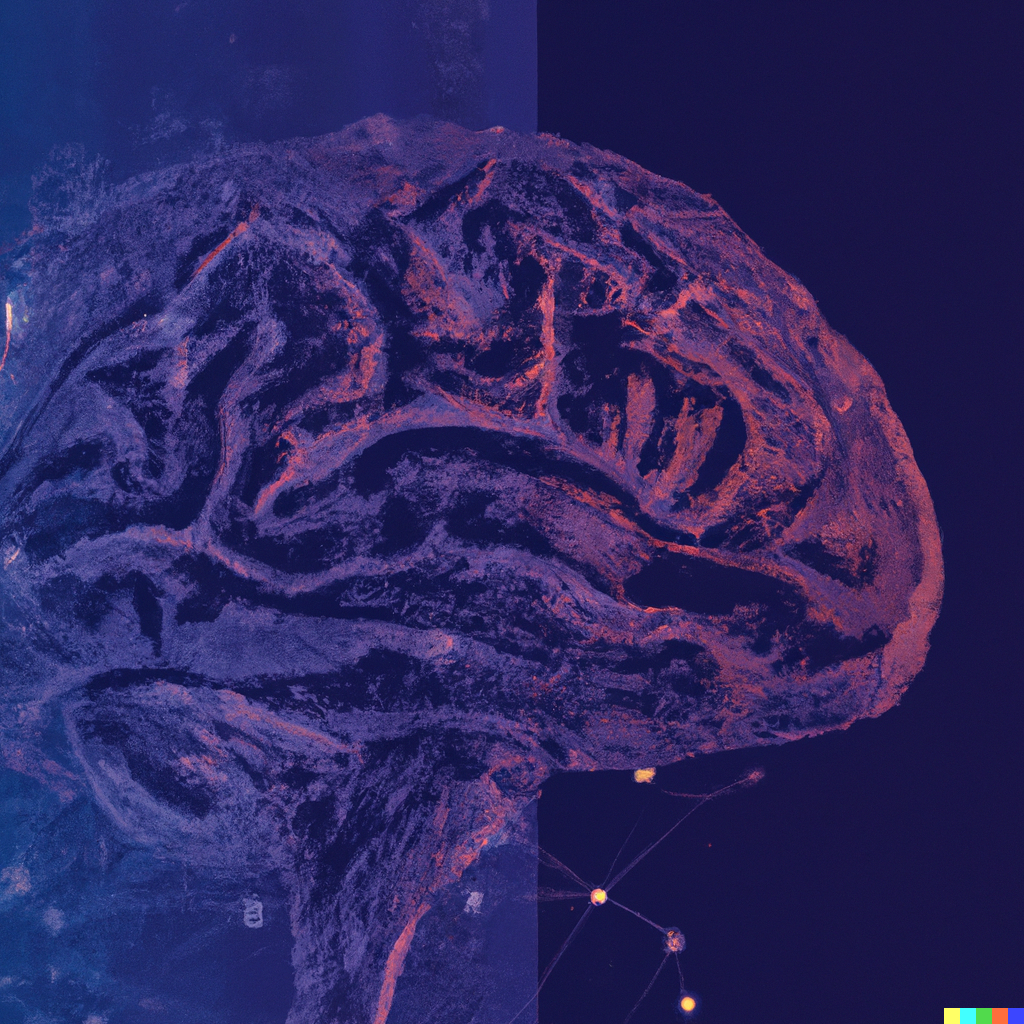
\includegraphics[width=0.7\textwidth, height=0.7\textheight, keepaspectratio]{dallecarso}
    \vspace*{10px}

    \texttt{[ \href{https://ballarin.cc/carsocode}{https://ballarin.cc/carsocode} ]}
\end{frame}
\end{document}
